\documentclass[11pt,a4paper]{article}

\usepackage[margin=2.3cm]{geometry}
\usepackage[T1]{fontenc}
\usepackage{lmodern}
\usepackage{amsmath,amssymb}
\usepackage{graphicx}
\usepackage{booktabs}
\usepackage{xcolor}
\usepackage{caption}
\usepackage{enumitem}
\usepackage{tikz}
\usetikzlibrary{arrows.meta,positioning,calc}
\usepackage[colorlinks=true,linkcolor=blue!50!black,urlcolor=blue!50!black,citecolor=blue!50!black]{hyperref}

\graphicspath{{figures/}}

% A figure from the repository root that may be missing in a fresh checkout.
\newcommand{\optionalfigure}[2]{%
  \IfFileExists{#1}{\includegraphics[width=#2]{#1}}%
  {\fbox{\parbox{0.8\linewidth}{\centering\small\vspace{2em}%
   Figure file \texttt{\detokenize{#1}} not found.\vspace{2em}}}}}

% Problem -> idea -> formulation: problem and idea side by side, the model in full width
\newcommand{\triple}[3]{%
  \par\medskip\noindent
  \begin{tabular}{@{}p{0.13\linewidth}@{\hspace{0.6em}}p{0.82\linewidth}@{}}
  \textbf{Problem} & #1\\[0.3em]
  \textbf{Idea}    & #2
  \end{tabular}\par\smallskip\noindent
  \textbf{Model.}\ #3\par\medskip}

\newcommand{\R}{\mathbb{R}}
\newcommand{\norm}[1]{\left\lVert #1 \right\rVert}
\newcommand{\Team}{\mathcal{T}}


\title{\textbf{More than a Hack 2027}\\[0.3em]
\large Ball possession and dead ball from tracking data:\\ FC Barcelona -- Athletic Club}
\author{Team tiki-taKA}
\date{17 November 2026}

\begin{document}
\maketitle

\begin{abstract}
\noindent
For every one of the 199{,}319 frames of the tactical video of FC Barcelona against Athletic
Club we decide whether Barcelona (\texttt{H}) or Athletic (\texttt{A}) has the ball, or
whether the ball is dead (\texttt{D}). The decision is made by rules on the data
supplied for the match -- the tracking of both cameras, the broadcast homography, the
published phase table and, as a cue, Smart Tagging's set pieces: no model
is trained on labels and no frame is annotated by hand. This document
explains each building block as a triple -- the \emph{problem} in the data, the
\emph{intuitive idea} that resolves it, and its \emph{mathematical formulation}. On the
public five-minute window the official scorer gives the submission a spellF1 of $0.526$
(published baselines $0.33$ and $0.42$) and a macroF1 of $0.737$. Its configuration -- including
the choice between two dead-ball logics we built -- was made on three labelled matches of other
games, Metrica's open sample data, as the rules ask.
\end{abstract}

\tableofcontents
\bigskip

%=====================================================================
\section{Introduction}
%=====================================================================

\emph{More than a Hack} is the hackathon of the Talent Arena Barcelona, organised with
FC~Barcelona -- \emph{m\'es que un club}, more than a club -- and Metrica Sports. The 2027
challenge is ball possession: given the tracking data of one complete match, label every
frame of its tactical video with the team in possession or with \emph{dead ball}.

The match is FC Barcelona against Athletic Club. Metrica supplies two recordings -- the
\emph{tactical} camera, a wide view that follows play, and the \emph{broadcast} -- each with
player and ball tracking at $25$ frames per second and, for the broadcast, a homography per
frame. The submission is one label per frame of the tactical video.

This document describes how our submission is produced. Section~\ref{sec:objective} states
the objective and the two scores. Section~\ref{sec:method} is the method, a sequence of
problem--idea--model triples in the order the pipeline runs them, with the alternatives we
built and compared. Section~\ref{sec:external} describes the labelled matches of other games on
which the settings were chosen, Section~\ref{sec:submitted} the submitted configuration,
Section~\ref{sec:results} the scores and Section~\ref{sec:rules} how the method keeps to the
rules.

%=====================================================================
\section{Objective}\label{sec:objective}
%=====================================================================

\paragraph{Labels.} Let $t\in\{0,\dots,N-1\}$, $N=199{,}319$, index the frames of the tactical
video. We predict $\hat y_t\in\{\texttt{H},\texttt{A},\texttt{D},\texttt{X}\}$: \texttt{H} --
Barcelona has the ball, \texttt{A} -- Athletic has it, \texttt{D} -- the ball is out of play,
\texttt{X} -- no answer. Only frames inside the published match phases are graded: the two
halves and the stretch before the second kickoff (which is all \texttt{D}).

\paragraph{macroF1 (tie-break).} With $\mathrm{P}_c$ and $\mathrm{R}_c$ the frame-wise
precision and recall of class $c$ over the graded frames,
\begin{equation}
  \mathrm{F1}_c = \frac{2\,\mathrm{P}_c\mathrm{R}_c}{\mathrm{P}_c+\mathrm{R}_c},\qquad
  \mathrm{macroF1} = \frac13\sum_{c\in\{\texttt{H},\texttt{A},\texttt{D}\}}\mathrm{F1}_c .
\end{equation}
Every frame counts the same, so it rewards being right most of the time.

\paragraph{spellF1 (ranking).} A \emph{spell} is a maximal run of frames with the same
possession label. Let $S$ be the true and $\hat S$ the predicted spells. A predicted spell
$\hat s$ matches a true spell $s$ of the same label if their intersection over union
\begin{equation}
  \mathrm{IoU}(\hat s,s)=\frac{|\hat s\cap s|}{|\hat s\cup s|}\ \ge\ \tau ,
\end{equation}
each spell matched at most once. With $m_\tau$ matches, precision $m_\tau/|\hat S|$ and recall
$m_\tau/|S|$ give $\mathrm{F1}_\tau$; the official scorer reports the mean over
$\tau\in\{0.3,0.4,0.5,0.6,0.7\}$. spellF1 judges \emph{episodes}, not frames: one brief
wrong change in the middle of a long possession splits it into pieces that each miss the
overlap threshold. It rewards timing changes of possession right and not flickering -- which
is why it ranks.

%=====================================================================
\section{Data and notation}
%=====================================================================

\begin{itemize}[leftmargin=1.2em]
\item Pitch $\Omega=[0,L]\times[0,W]$, $L=105.3$\,m, $W=68$\,m; tracking coordinates are
  delivered in $[0,1]^2$ and scaled to metres.
\item $P_i^t\in\Omega$: tactical position of player slot $i$ in frame $t$ (undefined where the
  player is out of the picture); $\Team(i)\in\{\texttt{H},\texttt{A}\}$ its team.
\item $Q_k^s$: broadcast position of player $k$ in broadcast frame $s$.
\item $b_t$: tactical ball position; $v_t=\lVert\dot b_t\rVert$ its speed by central differences.
\item Phases (published): first half from the kickoff at frame $11185$, second half from
  $113742$; before, between and after the halves nothing is graded except the stretch before
  the second kickoff.
\end{itemize}

\begin{figure}[ht]
\centering
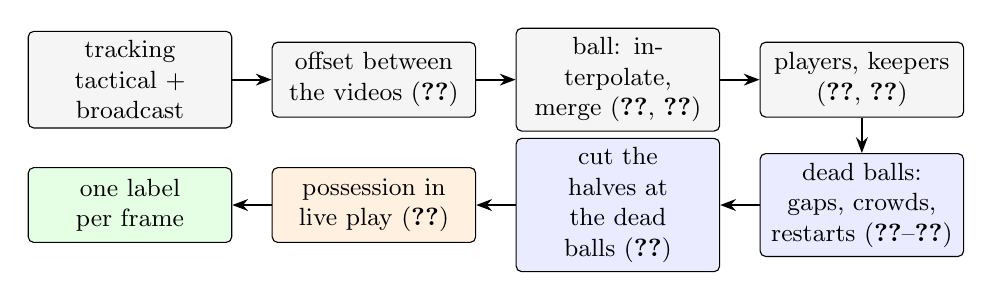
\begin{tikzpicture}[node distance=0.45cm and 0.5cm, every node/.style={font=\small},
  box/.style={draw, rounded corners=2pt, align=center, minimum height=0.95cm, text width=2.35cm, fill=#1},
  box/.default=gray!8, arr/.style={-{Stealth[length=2mm]}, thick}]
\node[box] (load) {tracking\\tactical + broadcast};
\node[box, right=of load] (sync) {offset between\\the videos (\ref{sec:offset})};
\node[box, right=of sync] (ball) {ball: interpolate,\\merge (\ref{sec:interp}, \ref{sec:merge})};
\node[box, right=of ball] (players) {players, keepers\\(\ref{sec:players}, \ref{sec:keeper})};
\node[box=blue!8, below=of players] (dead) {dead balls: gaps, crowds,\\restarts (\ref{sec:gaps}--\ref{sec:restarts})};
\node[box=blue!8, left=of dead] (cut) {cut the halves at\\the dead balls (\ref{sec:gaps})};
\node[box=orange!12, left=of cut] (poss) {possession in\\live play (\ref{sec:possession})};
\node[box=green!10, left=of poss] (out) {one label\\per frame};
\draw[arr] (load) -- (sync); \draw[arr] (sync) -- (ball); \draw[arr] (ball) -- (players);
\draw[arr] (players) -- (dead); \draw[arr] (dead) -- (cut); \draw[arr] (cut) -- (poss); \draw[arr] (poss) -- (out);
\end{tikzpicture}
\caption{The pipeline. Section numbers refer to the triples below.}
\label{fig:pipeline}
\end{figure}

%=====================================================================
\section{Method}\label{sec:method}
%=====================================================================

Every threshold below is a physical or football quantity (a running speed, a distance from
the Laws of the Game, a tracking accuracy) fixed in advance; only the three settings of the possession model (control radius, margin,
confirmation time) and the choice of the dead-ball logic were chosen by comparison with labels
-- of other matches (Section~\ref{sec:external}); all are listed in \texttt{development/config/config.yaml}.

%---------------------------------------------------------------------
\subsection{The offset between the two videos}\label{sec:offset}

\triple{The broadcast sees the ball where the tactical camera does not, but the two videos
run on different clocks: broadcast frame $s$ is not tactical frame $s$. Replays, cuts and the
almost missing halftime of the broadcast make the relation unclear.}
{Both videos record the same live match, and real time runs linearly. So within a half one
constant offset $\delta$ maps one clock onto the other. It can be found by recognising the
\emph{same pattern of player positions} in both: the moment the broadcast shows is the
tactical frame where the same players stand in the same places.}
{For a broadcast frame $s$ and a candidate tactical frame $t$ match each broadcast player to
the nearest tactical player of the same team, capped at $c=5$\,m so that one wrong player
cannot dominate:
\begin{equation}
 C(s,t)=\frac1{|K_s|}\sum_{k\in K_s}\min\Big(\min_{i:\,\Team(i)=\Team(k)}\norm{Q_k^s-P_i^t}^2,\ c^2\Big),
\end{equation}
summed over the frames $s,s+25,s+50$ (0, 1 and 2\,s) so that a still picture cannot match by
chance. For $400$ evenly spaced broadcast frames with a valid homography and at least $8$
players, $t^\ast(s)=\arg\min_t C(s,t)$. The offset of a half is the median
\begin{equation}
  \delta=\operatorname{median}_s\big(t^\ast(s)-s\big)
\end{equation}
after dropping the worst $5\,\%$ of matches; replays appear as outliers that match an
earlier moment. The model $t=s+\delta$ is accepted only if at least $85\,\%$ of the matches
lie within $0.5$\,s of it and the fitted slope differs from $1$ by less than $5\cdot10^{-4}$.
Result: $\delta=4014$ frames in the first half and $26919$ in the second; agreement
$99.5\,\%$ and $98.4\,\%$, slopes $0.99998$. The offsets are computed, never typed in.}

\begin{figure}[ht]
\centering
\optionalfigure{../../VersatzVideos.png}{0.85\linewidth}
\caption{Matched broadcast frames against their tactical frames. Live moments lie on one
line of slope one per half; replays fall off it.}
\label{fig:offset}
\end{figure}

%---------------------------------------------------------------------
\subsection{Short ball gaps: interpolation}\label{sec:interp}

\triple{The tactical tracker loses the ball for some frames: in duels, in the air, under a
player. Single frames are also false detections far from the true ball.}
{Over a few seconds the ball moves on smooth, nearly straight paths. A short gap can be
bridged by a straight line between where it was lost and where it is found again. A
detection that implies an impossible speed is not the ball.}
{A detection $b_t$ is removed if it implies a speed above $v_{\max}=40$\,m/s to both its
neighbours while these agree with each other. A gap $(t_0,t_1)$ with
$t_1-t_0\le 5\,\text{s}$ is filled linearly,
\begin{equation}
 b_t=b_{t_0}+\frac{t-t_0}{t_1-t_0}\,(b_{t_1}-b_{t_0}),\qquad t_0<t<t_1 ,
\end{equation}
and the velocity is the central difference $\dot b_t=(b_{t+2}-b_{t-2})/(4\Delta t)$. Gaps
are never bridged across the boundary of a match phase.}

%---------------------------------------------------------------------
\subsection{Long ball gaps: merging the two cameras}\label{sec:merge}

\triple{After interpolation the tactical ball still misses long stretches -- up to minutes
(Figure~\ref{fig:gaps}, top rows).}
{The broadcast may show the ball while the tactical camera does not. With the offset known,
its ball can be moved onto the tactical timeline -- but only where the broadcast shows the
match \emph{live}, not a replay or a close-up.}
{For a tactical gap longer than $5$\,s take the broadcast ball
$b_t:=\tilde b_{t-\delta}$ (pitch coordinates through the homography) wherever the broadcast
is live at $t-\delta$: the homography is valid with reprojection error at most $3$, and its
players match the tactical ones,
\begin{equation}
 \Big(\frac1{|K|}\sum_{k\in K}\min_{i:\,\Team(i)=\Team(k)}\norm{Q_k^{t-\delta}-P_i^t}^2\Big)^{1/2}\le 3\,\text{m},
 \qquad |K|\ge 4 .
\end{equation}
The merged ball is interpolated again as in Section~\ref{sec:interp}.}

\begin{figure}[p]
\centering
\includegraphics[width=\linewidth]{ball_gaps_first_half.png}\\[0.5em]
\includegraphics[width=\linewidth]{ball_gaps_second_half.png}
\caption{Frames since the ball was last seen, first (top) and second half (bottom); left over
the video frame, right over the match minute. Rows: tactical camera, broadcast (on its own
clock above), merged (orange: ball taken from the broadcast), and the long gaps that remain,
judged dead (red) or unclear (grey). The dashed line is the $5$\,s up to which gaps are
interpolated.}
\label{fig:gaps}
\end{figure}

%---------------------------------------------------------------------
\subsection{What remains unseen is mostly a dead ball}\label{sec:gaps}

\triple{Even after merging, gaps longer than $5$\,s remain. Is play going on unseen, or has it
stopped?}
{The tactical tracker loses the ball mostly when play stops: the ball goes out, players walk,
the broadcast cuts to replays. Practically all its gaps are either under $1$\,s or longer than
$5$\,s, and the long ones cover about $40\,\%$ of the graded frames -- close to the share of a
professional match in which the ball is out of play. The players show it: when the referee
stops play, they stop running.}
{This is the dead-ball logic of the submission (\emph{gap-based}). Let
$\bar v(t)=\operatorname{median}_i\norm{\dot P_i^t}$ be the median player speed. Each gap
$G=(t_0,t_1)$ of at least $5$\,s of the \emph{tactical} ball -- a broadcast ball glimpsed during
a stoppage must not hide it -- is judged:
\begin{itemize}[leftmargin=1.2em]
\item \emph{keeper hold}: the same goalkeeper controls the ball where it vanishes and where it
  reappears, and it was not last seen at a line -- a catch is play (Law 12), his team has it;
\item \emph{dead}: the ball was last seen out of play, $b_{t_0-1}\notin\Omega^{+1.5}$ (more than $1.5$\,m beyond a line); or
  the players walk, $\operatorname{median}_{t\in G}\bar v(t)\le 1.5$\,m/s; or they are slow,
  $\le 2.0$\,m/s, and one more cue agrees: the ball last seen at a line, reappearing at a restart
  spot $b_{t_1}\in\mathcal R$, a crowd episode (Section~\ref{sec:crowd}) or a Smart Tagging set
  piece around the restart -- a tag never decides alone;
\item \emph{live} otherwise: play goes on unseen and the owner keeps the ball.
\end{itemize}
Here $\Omega^{+1.5}$ is the pitch enlarged by $1.5$\,m (the tracking accuracy of the ball); ``at a
line'' means outside the pitch shrunk by $1.5$\,m, $\mathcal R$ the
restart spots (corner arcs, goal areas, touchlines, centre and penalty spot); walking pace is
about $1.4$\,m/s. Also dead: the observed ball more than $1.5$\,m beyond a line for at least
$0.4$\,s; the waiting before an accepted placed-ball restart (Section~\ref{sec:restarts}); the
graded frames before a half's kickoff (Law 8).}

%---------------------------------------------------------------------
\subsection{Players: bridging lost tracks}\label{sec:players}

\triple{A player's track breaks off when he leaves the picture and comes back under a new
track number; at any moment only about $22$ of the $46$ track slots are filled.}
{A player cannot run faster than a sprinter. A track that ends and another of the same team
that starts within reach of it belong to the same player; players missing in the tactical
view may be visible in the broadcast.}
{A track ending at $(P_e,t_e)$ is linked to one starting at $(P_s,t_s)$ of the same team if
\begin{equation}
  0<t_s-t_e\le 10\,\text{s},\qquad \norm{P_s-P_e}\le 7\,\tfrac{\text{m}}{\text{s}}\,(t_s-t_e)+2\,\text{m},
\end{equation}
links taken greedily by increasing cost $\norm{P_s-P_e}$ (plus $2$\,m for a change of
track), and the gap filled linearly. Where a team has fewer than $11$ players and the
broadcast is live, broadcast players more than $3$\,m from every tactical teammate are added.
The keeper slots are only ever linked to themselves.}

%---------------------------------------------------------------------
\subsection{Goalkeepers: the deepest player}\label{sec:keeper}

\triple{The tactical camera follows play, so the keeper at the far end is out of the
picture most of the time.}
{The keeper is his team's deepest player and never leaves his half. Unseen, he stays where
he was last seen -- he hardly moves while play is far away.}
{The goal $g\in\{0,L\}$ a team defends follows from its centre in the second before the
kickoff (all players stand in their own half). Per frame and team the keeper is
\begin{enumerate}[leftmargin=1.5em, label=(\roman*)]
\item the keeper track of the metadata, if it is in its own half: $|x-g|\le L/2$;
\item else the deepest player $i^\ast=\arg\min_i|x_i-g|$, if he stands in his own penalty box
  and $|x_{(2)}-g|-|x_{i^\ast}-g|\ge 5$\,m (clearly behind the next teammate -- otherwise he
  is the last defender while the keeper is out of view);
\item else held at his last seen position in this half.
\end{enumerate}
Held positions are not measurements: the dead-ball indicators leave them out.}

%---------------------------------------------------------------------
\subsection{Dead balls from crowding and speed}\label{sec:crowd}

\triple{Not every stoppage hides the ball. Corners, free kicks with a wall, goal
celebrations and cooling breaks happen with the ball in view.}
{At such stoppages the players crowd together -- into the box, around the wall, at the
bench -- and they slow down. The densest spot of the pitch and the median speed mark them.}
{The crowd of frame $t$ is the largest number of players in a circle of radius $r=10$\,m
around one of them,
\begin{equation}
  \kappa(t)=\max_i\ \big|\{\,j:\ \norm{P_j^t-P_i^t}\le r\,\}\big| ,
\end{equation}
and a crowd episode is a stretch of at least $3$\,s with $\kappa\ge 12$ (rolling median over
$1$\,s). Together with $\bar v(t)$ it is one of the cues by which the long ball gaps above are
judged.}

%---------------------------------------------------------------------
\subsection{Restarts: which set piece, which team}\label{sec:restarts}

\triple{A stoppage ends with a restart: a corner, a throw-in, a goal kick, a free kick, a
kickoff, a penalty. Its kind and its team say who has the ball when play resumes.}
{Before a restart the ball lies still at a place the Laws prescribe, and the opponents must
stand back. Where it lies tells the kind; the kind tells the team -- by the goal at that end
or by the taker at the ball.}
{A \emph{candidate} is a stretch of at least $1$\,s with the ball still (rolling median of
$v_t$ at most $1.5$\,m/s); it is played at its last frame $t_p$. At $b_{t_p}$, in this
order:
\begin{center}\small
\begin{tabular}{@{}lll@{}}
\toprule
kind & where the ball lies & team \\ \midrule
corner & within $2.5$\,m of a corner flag & attacking that goal \\
goal kick & in a goal area & defending that goal \\
throw-in & within $1.5$\,m of a touchline (or up to $3$\,m beyond) & the taker's \\
kickoff & within $1.5$\,m of the centre spot & the taker's \\
penalty & within $1.5$\,m of a penalty spot & attacking that goal \\
keeper holds & elsewhere, a keeper nearest & his (play goes on) \\
free kick & elsewhere & the taker's \\ \bottomrule
\end{tabular}
\end{center}
The taker is the nearest player $i^\ast$ at $t_p$. A candidate is a \emph{restart} only if
\begin{equation}
  t_p-t_0\ \ge\ \tau_{\text{kind}},\qquad
  \min_{j:\,\Team(j)\neq\Team(i^\ast)}\norm{P_j^{t_p}-b_{t_p}}\ \ge\ d_{\text{kind}},\qquad
  \operatorname{median}_{t\in[t_0,t_p]}\bar v(t)\le 2\,\text{m/s},
\end{equation}
with $\tau=1$\,s for a kickoff, $2$\,s for a throw-in and $3$\,s for the others, and $d$
below the Laws' $2$\,m (throw-in) and $9.15$\,m (others) for tracking error and quick restarts.
Three more tests came from watching the video and the tracking of the provided game where
candidates were wrong -- inspecting the data to design features, as the rules allow; none refers
to a particular frame, and none changes a frame of the public window:
\begin{itemize}[leftmargin=1.2em]
\item \emph{A free kick has a foul before it:} in the $10$\,s before the ball comes to rest an
  opponent of the taker was within $2$\,m of the ball. A player holding the ball in the
  build-up has the opponents far away all along.
\item \emph{A penalty has its scene:} in the last $2$\,s at most one player besides the
  keepers is in the box and the players do not run off -- both as medians over the players and the $2$\,s: at most one
  field player in the box, and a speed away from the penalty spot of at most $1$\,m/s. A keeper holding
  the ball in his box, with everybody running upfield for the throw-out, is play.
\item \emph{A throw-in may be unseen} -- the ball held over the head: a player standing still
  at least $0.3$\,m behind a touchline for at least $1$\,s (his own speed at most $1.5$\,m/s), then passing the throw-in tests above
  (at least $2$\,s, nearest opponent $1.5$\,m away, players' median speed at most $2$\,m/s), the ball (where seen) at a median distance of at most $5$\,m, back on the pitch within $3$\,s.
\end{itemize}
The submission uses the restarts in two ways: an \emph{accepted} restart -- its taker within the
control radius of Section~\ref{sec:possession}, its team not contradicting the goal at that end,
the ball then seen moving -- makes the waiting before it dead, and gives the team that restarts
play.}

%---------------------------------------------------------------------
\subsection{Alternative: where a stoppage begins, and catches}\label{sec:cut}

\noindent This part belongs to the second, \emph{restart-based} dead-ball logic, which we built and
compared but did not submit (Section~\ref{sec:compare}).

\triple{A restart marks the \emph{end} of a stoppage. The label \texttt{D} starts earlier --
when the ball goes out or the whistle blows -- and a keeper's catch, though the ball vanishes
in his arms, is no stoppage at all (Law 12).}
{Look back from the ball at rest: the stoppage began where the ball crossed a line, or else
where the players fell to walking pace. A long gap that begins at the keeper -- or ends with
the ball flying out of a penalty box -- is the keeper holding it.}
{A dead-ball event is a restart or a dead gap; overlapping ones (within $1$\,s) are merged.
Its start, looking back at most $60$\,s and never past the event before:
\begin{equation}
 t_{\text{start}}=
 \begin{cases}
  \min\{t:\ b_t\notin\Omega^{+1.5}\ \text{for}\ \ge0.4\,\text{s}\}\ \text{(runs $<3$\,s apart joined)}, & \text{if the ball was out},\\
  \min\{t:\ \bar v(t')\le 1.5\ \forall t'\in[t,t_0]\}-1\,\text{s}, & \text{else if players walk},\\
  t_0, & \text{else},
 \end{cases}
\end{equation}
and the dead ball is $[t_{\text{start}},t_p]$. A long gap not last seen out of play is a
\emph{catch} if the ball vanished within $2$\,m of a keeper, or if it reappears in flight
($\ge 5$\,m/s) and, run back along its flight,
\begin{equation}
 b_{t_1}-\lambda\,\frac{\dot b_{t_1}}{\norm{\dot b_{t_1}}}\ \in\ \text{penalty box of team }T
 \quad\text{for some }0\le\lambda\le 60\,\text{m}
\end{equation}
-- team $T$'s keeper caught it unseen and threw it out. The keeper's tracked position is not
used here: out of the picture it is only where he was last seen, often far off. Figure
\ref{fig:catch} sketches the test; Figure~\ref{fig:dead} shows the resulting dead balls.}

\begin{figure}[ht]
\centering
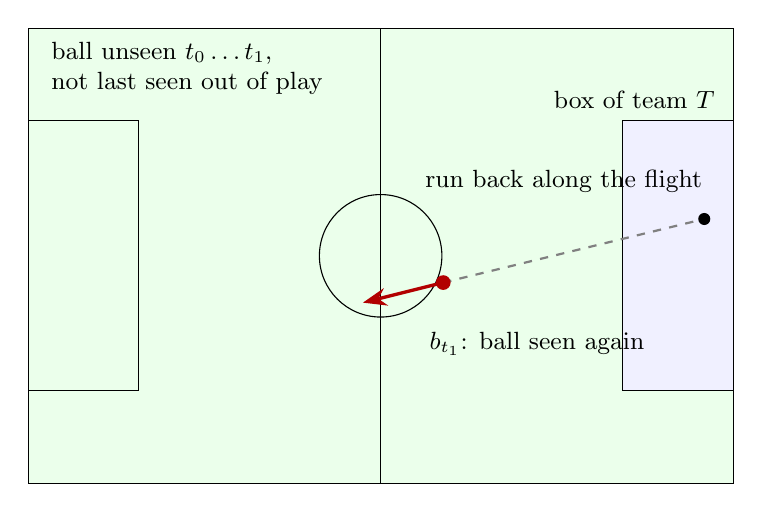
\begin{tikzpicture}[scale=0.085, every node/.style={font=\small}]
\draw[fill=green!8] (0,0) rectangle (105.3,68);
\draw (52.65,0) -- (52.65,68); \draw (52.65,34) circle (9.15);
\draw[fill=blue!6] (105.3,13.84) rectangle (88.8,54.16);
\draw (0,13.84) rectangle (16.5,54.16);
\node[anchor=south east] at (104,54.5) {box of team $T$};
\draw[dashed, thick, gray] (62,30) -- (101,39.5);
\fill (101,39.5) circle (0.9) node[right] {};
\draw[-{Stealth[length=3mm]}, very thick, red!70!black] (62,30) -- (50,27);
\fill[red!70!black] (62,30) circle (1.1);
\node[below] at (76,24) {$b_{t_1}$: ball seen again};
\node[above, align=center] at (80,42) {run back along the flight};
\node[align=left, anchor=west] at (2,62) {ball unseen $t_0\ldots t_1$,\\ not last seen out of play};
\end{tikzpicture}
\caption{A catch seen only afterwards: the ball turns up in flight; run back along its flight
it comes out of the box of team $T$, so $T$'s keeper had it -- play, not a dead ball.}
\label{fig:catch}
\end{figure}

%---------------------------------------------------------------------
\subsection{Two dead-ball logics compared}\label{sec:compare}

Two logics for \texttt{D} were built and compared over the whole match
(Figure~\ref{fig:dead}). Both use the same inputs; they differ in what they take as the
\emph{core} of a stoppage and in how they find its boundaries.

\begin{center}\small
\begin{tabular}{@{}p{0.2\linewidth}p{0.36\linewidth}p{0.36\linewidth}@{}}
\toprule
 & \textbf{gap-based} (\texttt{stoppages.py}) & \textbf{restart-based} (\texttt{segments.py}) \\ \midrule
core of a stoppage & a long gap ($\ge 5$\,s) of the \emph{tactical} ball, judged by the players' pace
  (Section~\ref{sec:gaps}) & a restart: the ball lying still, then played, with its kind and team
  (Section~\ref{sec:restarts}) \\[0.3em]
further dead ball & ball clearly beyond a line for $0.4$\,s; the waiting before an accepted
  placed-ball restart; frames before a kickoff & long gaps of the \emph{merged} ball judged dead
  (Section~\ref{sec:gaps}), merged with the restarts \\[0.3em]
where it begins & where the tactical ball vanishes & looking back: where the ball crossed a line,
  else where the players fell to walking pace (Section~\ref{sec:cut}) \\[0.3em]
where it ends & where the ball reappears & where the restart is played \\[0.3em]
keeper with the ball & the same keeper at the ball where it vanishes and reappears & the ball
  vanishes at a keeper, or turns up flying out of a penalty box (Section~\ref{sec:cut}) \\[0.3em]
strength & robust where the ball is unseen; never mistakes calm build-up for a stoppage & sees
  stoppages with the ball in view; starts them when play stops, not when the camera loses the ball \\[0.3em]
weakness & a stoppage with the ball in view begins late or is missed & depends on still-ball
  candidates; a quick restart may be missed \\ \bottomrule
\end{tabular}
\end{center}

\noindent
The two were compared where the rules allow a choice: on labelled matches of other games
(Section~\ref{sec:external}), under the same possession model. The gap-based logic is better on
all three matches and under both label definitions (spellF1 $0.527$ against $0.489$, and $0.629$
against $0.581$), and so is its alive/dead F1 ($0.959$ against $0.934$). Switching off single
building blocks showed where the restart-based logic lost: its looked-back start of a stoppage.
One suspect was its ball-out test, which took a ball tracked more than $0.5$\,m beyond a line in a
single frame as out -- the tracking error of the ball near a line can trigger that.
Requiring, as the gap-based logic does, $1.5$\,m for at least $0.4$\,s changes the
restart-based logic alone little ($0.486\to0.489$; the looked-back start still costs about
$0.012$), but it makes the merge below level with the gap-based logic ($0.504\to0.526$), since
that merge trusts observed balls out.

We then merged the two by a rule fixed beforehand: per stoppage, the logic with the richer data
there -- the restart-based one where the tracked ball is seen crossing a line, or a placed ball is
seen where the other sees no stoppage; the gap-based one where the ball is unseen and only the
players' pace can tell; nothing where only the restart-based one sees a stoppage, from walking
pace or a ball gap alone. On the sample matches this choice is level with the gap-based logic alone ($0.526$
against $0.527$, and $0.629$ against $0.629$), better on one match and worse on two
(Table~\ref{tab:benchmark}). By the rule we set before -- a change must win on average and on at
least two of three matches, a tie goes to the simpler -- the submission uses the gap-based logic.
It relies itself on the restart recognition of Section~\ref{sec:restarts} (accepted restarts and
their teams) and on the crowd episodes of Section~\ref{sec:crowd}. The choice by evidence is a
switch in the code (\texttt{baseline.dead: evidence}); on a match with a broadcast, which the
sample matches lack, it may well be the better one.

\begin{figure}[p]
\centering
\includegraphics[width=\linewidth]{dead_balls_first_half.png}\\[0.6em]
\includegraphics[width=\linewidth]{dead_balls_second_half.png}
\caption{Dead balls over the first (top) and second half (bottom); left over the video frame,
right over the match minute. Rows: the gap-based logic (used for the submission), the
restart-based logic (compared, Section~\ref{sec:compare}) and, in the first half, the public ground truth's \texttt{D} in its five minutes.
Each bar is one dead ball, coloured by its kind; \textbf{white is live play}. Colours:
\textcolor[HTML]{2a78d6}{\rule{0.8em}{0.8em}}~throw-in,
\textcolor[HTML]{eb6834}{\rule{0.8em}{0.8em}}~corner,
\textcolor[HTML]{1baf7a}{\rule{0.8em}{0.8em}}~goal kick,
\textcolor[HTML]{eda100}{\rule{0.8em}{0.8em}}~free kick,
\textcolor[HTML]{e87ba4}{\rule{0.8em}{0.8em}}~kickoff,
\textcolor[HTML]{008300}{\rule{0.8em}{0.8em}}~penalty,
\textcolor[HTML]{6250d6}{\rule{0.8em}{0.8em}}~other (no restart recognised: a free kick without
a still ball, an injury, a drinks break),
\textcolor[HTML]{6b7280}{\rule{0.8em}{0.8em}}~\texttt{D} of the ground truth (it has no kind).
The kind is found the same way for both logics: from a recognised restart at the end of the
dead ball, else from where the ball is first seen within $1$\,s after it (corner flag, goal
area, touchline, centre spot), else \emph{other}.}
\label{fig:dead}
\end{figure}

%---------------------------------------------------------------------
\subsection{Possession in live play}\label{sec:possession}

\triple{Between two dead balls play is live. Who has the ball -- at the restart and after every
change in open play?}
{After a restart the team of the taker has the ball. In open play a team has the ball when
one of its players is at it, clearly nearer than any opponent. Possession changes only when
the other team keeps it for a moment -- a touch or a deflection is no change -- and otherwise
stays with the last team that had it, through passes, loose balls and unseen stretches.}
{Each half is cut into dead balls (label \texttt{D}, Section~\ref{sec:gaps}) and live
stretches between them. A live stretch starts with the restarting team: that of an accepted
placed-ball restart released at its start; else, from the first ball seen within $1$\,s, at a
corner flag the attacking team, in a goal area the defending team, elsewhere the player in
control by the test below (the taker); else the first team whose control is confirmed in it.
In the stretch, with $d_T(t)$ the distance of team
$T$'s nearest player to the ball, frame $t$ is evidence for $T$ if
\begin{equation}
  b_t\ \text{observed},\qquad v_t\le 12\,\text{m/s},\qquad d_T(t)\le 3\,\text{m},\qquad
  d_T(t)+1\,\text{m}<d_{T'}(t)\quad(T'\neq T).
\end{equation}
The label is a two-state process: the owner keeps the ball until the other team has
evidence on $0.6$\,s of consecutive frames; the change is then dated back to the first of
them (the prediction is offline). A keeper holding the unseen ball (Section~\ref{sec:gaps})
gives his team the ball for as long as he holds it. The $3$\,m radius, $1$\,m margin and $0.6$\,s confirmation
were chosen on Metrica's labelled open sample matches -- other games -- with ball noise
matched to this match.}

\begin{figure}[ht]
\centering
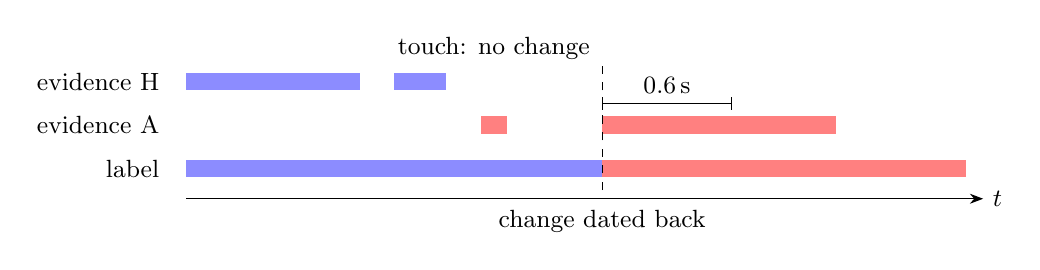
\begin{tikzpicture}[x=0.11cm, y=0.55cm, every node/.style={font=\small}]
\foreach \y/\lab in {2/evidence H, 1/evidence A, 0/label}{\node[anchor=east] at (-2,\y) {\lab};}
\fill[blue!45] (0,1.8) rectangle (20,2.2); \fill[blue!45] (24,1.8) rectangle (30,2.2);
\fill[red!50] (34,0.8) rectangle (37,1.2); \fill[red!50] (48,0.8) rectangle (75,1.2);
\fill[blue!45] (0,-0.2) rectangle (48,0.2); \fill[red!50] (48,-0.2) rectangle (90,0.2);
\draw[-{Stealth}] (0,-0.7) -- (92,-0.7) node[right] {$t$};
\draw[|-|] (48,1.5) -- (63,1.5); \node[above] at (55.5,1.5) {$0.6$\,s};
\draw[dashed] (48,-0.5) -- (48,2.4);
\node[above] at (35.5,2.3) {touch: no change};
\node[below] at (48,-0.75) {change dated back};
\end{tikzpicture}
\caption{Possession as a two-state process: a short touch of the other team changes nothing;
$0.6$\,s of its evidence does, from the first frame of it.}
\end{figure}

%---------------------------------------------------------------------
\subsection{Why this possession model}\label{sec:whymodel}

Our first rule for open play was stricter: a change only after the other team kept a player
within $1$\,m of the ball for $2$\,s without a break. Looking at the result over the whole match
showed what that does -- it produced only $106$ possessions in the match, about a third of the submission's $346$, and
missed most short possessions: a ball won, passed once and lost again never qualifies, though it
is a real possession. Football agrees: a possession often consists of a few touches of under a
second each, and the ball is controlled at the feet, not on top of the player's tracked centre.

The rule was therefore replaced by the model of Section~\ref{sec:possession} (radius $3$\,m, margin
$1$\,m, confirmation $0.6$\,s), whose settings were chosen on three independent labelled matches
(Section~\ref{sec:external}). On them the settings degrade steadily towards the strict end --
radius $1.5$\,m gives spellF1 $0.414$ instead of $0.527$, confirmation $1.2$\,s $0.446$ -- and our
first rule, run there as well, scores $0.14$ against $0.53$. On the provided game the model predicts $346$ possessions in the match instead of $106$.

The reason to prefer a choice made this way is \emph{generality}. A setting chosen on one match --
let alone on its five public minutes, $17$ possessions -- fits that match's quirks; a setting that
holds on three other matches, with about $270$--$380$ possessions each and the ball error of the
challenge simulated, describes how possession works in football as tracked by Metrica. That is
what the rules ask for: a system that would work on the next match.

%---------------------------------------------------------------------
\subsection{An idea we explored: block shifts}

\triple{In build-up play the ball is mostly in view, but the camera may lose it, and the
nearest player is not always the one in control.}
{The defending team shifts with the ball as one block -- everybody moves by the same vector
and the shape stays -- while the team in possession spreads out.}
{With $\Delta P_i=P_i^{t+h}-P_i^{t-h}$ over $2h=2$\,s, the common shift of a team and its
rigidity are
\begin{equation}
  c(t)=\operatorname{median}_i\Delta P_i,\qquad
  \rho(t)=\frac{\norm{c}}{\norm{c}+\operatorname{median}_i\norm{\Delta P_i-c}}\in[0,1],
\end{equation}
a block shift being $\norm{c}\ge 3$\,m, $\rho\ge 0.7$ with at least $7$ players
(Figure~\ref{fig:blocks}). The signal is clear in single moments but symmetric -- on a switch
of play both teams shift -- and it lags a change of possession by about $3$\,s, so it is not
part of the submission.}

\begin{figure}[ht]
\centering
\includegraphics[width=\linewidth]{block_shifts.png}
\caption{Common shift $\lVert c\rVert$ and rigidity $\rho$ per team (blue H, red A) over both
halves; shaded where a team shifts as a block. Bottom strip of the first panel: the public
ground truth's five minutes, for understanding only.}
\label{fig:blocks}
\end{figure}

%=====================================================================
\section{External data: labelled matches of other games}\label{sec:external}
%=====================================================================

\paragraph{Why.} Every method has settings -- a control radius, a confirmation time, which
dead-ball logic to use. The rules forbid choosing them on the provided game: no hand labels on
it for any purpose, and the public five minutes are not a tuning set. Labelled data of
\emph{other} games is allowed in any amount. So every choice between settings was made there.

\paragraph{What.} Metrica Sports' open sample data
(\url{https://github.com/metrica-sports/sample-data}): three anonymised professional matches with
tracking of all players and the ball at $25$\,fps -- the provider, formats and frame rate of the
challenge -- and event data annotated by Metrica (passes, shots, fouls, balls out, \dots). We
labelled nothing ourselves. From the events, labels per frame are derived by code
(\texttt{src/external.py}): the team of the latest on-ball event has the ball (\emph{touch});
the ball is dead from a ball out, goal, offside, foul or referee stop until the next on-ball
event. A \emph{controlled} variant applies the control proxies of the challenge: a possession won
in open play counts only if it lasts $2$\,s or contains a completed pass.

\paragraph{How.} Each match runs through the unchanged submission code
(\texttt{src.baseline.prepare}/\texttt{decode}) and is scored with the official metric library
(\texttt{src.benchmark}). The sample tracking is corrected and far cleaner than the challenge
input -- its ball lies $0.1$\,m from its owner, against a median of $1.8$\,m between ball and
nearest player in the challenge's live play -- so a smooth ball error ($1.15$\,m per axis,
$3$\,s time constant), measured on the challenge input without labels, is added. The sample
matches have no broadcast and no Smart Tagging.

\begin{table}[ht]
\centering\small
\resizebox{\linewidth}{!}{%
\begin{tabular}{@{}lcccc@{}}
\toprule
 & \multicolumn{2}{c}{spellF1, mean of 3 matches} & alive/dead F1 & team acc. \\
 & touch & controlled & & \\ \midrule
\textbf{submitted: gap-based D, $3$\,m, $1$\,m, $0.6$\,s} & \textbf{0.527} & \textbf{0.629} & \textbf{0.959} & \textbf{0.869} \\
confirmation $0.4$\,s / $0.8$\,s & 0.520 / 0.497 & 0.584 / 0.625 & 0.960 & \\
control radius $2$\,m / $4$\,m & 0.465 / 0.526 & 0.582 / 0.617 & 0.959 & \\
margin $0.5$\,m / $2$\,m & 0.520 / 0.476 & 0.596 / 0.610 & 0.960 & \\
no restart team & 0.484 & 0.584 & 0.953 & \\
team-shape stage & 0.528 & 0.633 & 0.960 & \\ \midrule
restart-based D (Section~\ref{sec:cut}) & 0.489 & 0.581 & 0.934 & 0.866 \\
union of both, start looked back only from an observed ball out & 0.507 & 0.607 & 0.957 & \\
per stoppage the logic with the richer data there & 0.526 & 0.629 & 0.958 & 0.869 \\ \midrule
oracle: true dead balls / true team in live play & 0.554 / 0.933 & 0.663 / 0.924 & 1.000 / 0.959 & \\ \bottomrule
\end{tabular}}
\caption{Benchmark on Metrica's three sample matches with challenge-like ball noise. The
submitted settings are best or within $0.005$ of the best under both label definitions; the
team-shape stage gains $0.001$--$0.004$, not consistently over the matches, and stays off. The
oracles replace one component by the truth: perfect dead balls would add about $0.03$, perfect
team calls in live play about $0.3$ -- possession in open play is where the remaining error is.}
\label{tab:benchmark}
\end{table}

%=====================================================================
\section{The submitted configuration}\label{sec:submitted}
%=====================================================================

\begin{center}
\fbox{\parbox{0.92\linewidth}{\small
\textbf{Submitted:} \texttt{baseline.dead: gap}, \texttt{baseline.possession: stefan}, team shape off.
\begin{itemize}[leftmargin=1.2em, itemsep=0pt]
\item \emph{Dead ball} (Section~\ref{sec:gaps}): long tactical ball gaps judged by the players'
  pace, the ball clearly out, the waiting before an accepted restart (Section~\ref{sec:restarts}),
  the frames before a kickoff; crowd episodes (Section~\ref{sec:crowd}) and Smart Tagging set
  pieces as cues that never decide alone.
\item \emph{Possession} (Section~\ref{sec:possession}): control within $3$\,m and $1$\,m nearer than
  every opponent, a change after $0.6$\,s, the restarting team at the start of live play.
\item \emph{Inputs}: tactical and broadcast tracking, broadcast homography, the published phase
  table, Smart Tagging set pieces. The videos are not used.
\end{itemize}
\textbf{Built, compared and not submitted} (switches in the code): the restart-based dead ball
(\texttt{restart}), dead where either logic says so (\texttt{union}), both judged per kind of
restart (\texttt{combined}), the logic with the richer data per stoppage (\texttt{evidence}, level
with the submission on the sample matches), our first possession rule (Section~\ref{sec:whymodel}),
the team-shape stage, and block shifts (Figure~\ref{fig:blocks}). As a diagnostic we also checked
Smart Tagging's set-piece tags against the tracking (is the mark of the claimed set piece really
there?) -- useful to look at, not used for the labels.}}
\end{center}

%=====================================================================
\section{Results}\label{sec:results}
%=====================================================================

The public ground truth covers five minutes of the first half (7{,}500 graded frames, 17
possessions). It was used to check the pipeline and to look at situations; no setting was chosen
on it. With so few possessions the scorer's bootstrap band of the spellF1 is about $0.3$ wide
(below): differences smaller than that say nothing.

\begin{table}[ht]
\centering
\begin{tabular}{@{}lccc@{}}
\toprule
 & spellF1 & macroF1 & alive/dead F1 \\ \midrule
published baseline \texttt{smooth50}  & 0.33 & -- & -- \\
published baseline \texttt{smooth125} & 0.42 & -- & -- \\
\textbf{submission} (gap-based dead ball, Section~\ref{sec:possession}) & \textbf{0.526} & \textbf{0.737} & \textbf{0.916} \\
alternative: restart-based dead ball, same possession model & 0.546 & 0.805 & 0.939 \\ \bottomrule
\end{tabular}
\caption{Public five minutes, official scorer. The bootstrap band of the submission's spellF1
is $0.37$--$0.66$.}
\end{table}

Further numbers of the official scorer for the submission: frame-wise F1 $0.857$ for
\texttt{H}, $0.802$ for \texttt{A} and $0.552$ for \texttt{D}; $18$ predicted possessions against
$17$ true, of mean duration $14.6$\,s against $14.2$\,s; F1 of the transition times $0.29$ within
$\pm 1$\,s. Most frame errors in the window are dead-ball frames labelled live (\texttt{D} recall
$0.45$): stoppages that begin while the ball is still visible start late. Over the whole match
the submission marks $41.8\,\%$ of the graded frames dead in $141$ stoppages and predicts $346$
possessions.

%=====================================================================
\section{Rules and reproducibility}\label{sec:rules}
%=====================================================================

\begin{itemize}[leftmargin=1.2em]
\item \textbf{No labels of the provided game for training or tuning.} Nothing is fitted to it;
  the public five minutes were only used to check the pipeline and look at situations.
  Thresholds are football and physical quantities; choices between settings were made on
  Metrica's open sample matches, other games (Section~\ref{sec:external}). The optional
  team-shape stage, off in the submission, would fit a small model per match on the pipeline's
  own pseudo-labels -- no person decides any of them.
\item \textbf{No hand annotation, no frame constants.} Every label comes from code; no
  threshold refers to a particular frame. The phase boundaries are the published phase table.
\item \textbf{No typed-in offsets.} The broadcast offsets are computed
  (Section~\ref{sec:offset}) and accepted only after the consistency checks.
\item \textbf{Reproducible.} The submission is written by \texttt{python -m src.baseline}, run in
  \nolinkurl{development/}, to \nolinkurl{outputs/BAR-ATH_baseline.csv}, with
  \texttt{baseline.dead: gap} in \nolinkurl{config/config.yaml}; it runs the same chain as
  \nolinkurl{run_pipeline.py} in the repository root. The official validator
  \nolinkurl{evaluation/validate_submission.py} accepts it ($199{,}319$ rows).
  Parsed tracking and alignments are cached by the contents of the inputs and of the parsing
  code; a run gives the same file.
\item \textbf{Data stays private.} Tracking, labels, caches and outputs are git-ignored and not
  published.
\end{itemize}

%=====================================================================
\section{Limitations and outlook}
%=====================================================================

\begin{itemize}[leftmargin=1.2em]
\item \textbf{Changes of possession in open play} are the largest error: duels, one-touch play
  and long passes between opponents give late or wrong changes (transition F1 $0.29$; the
  oracle of Table~\ref{tab:benchmark} puts the potential there).
\item \textbf{Dead-ball boundaries.} Dead ball is inferred from when the tactical tracker loses
  the ball and how the players move: a stoppage with the ball in view starts late, at its
  disappearance, and slow live play the camera cannot follow can be taken for a stoppage. Our
  restart-based logic addresses the first, but did not beat the gap-based one on the sample
  matches, which have no broadcast to help it.
\item \textbf{Keeper positions out of the picture} are only where he was last seen.
\item \textbf{Validation.} Five public minutes cannot establish full-match quality, and the
  sample matches are other games with corrected tracking, simulated ball error and labels
  derived from events, not from the challenge's definition. More labelled matches -- ideally with
  a broadcast -- would make the choices firmer.
\end{itemize}

\end{document}
